\section{Theoretical Background}

All phylogenetic methods make assumptions, whether explicit or implicit, about the process of DNA substitution \citep{Felsenstein-1988}. Consequently, all the methods of phylogenetic inference depend on their underlying substitution models. To have confidence in inferences it is necessary to have confidence in the models \citep{Goldman-1993b}. Because of this, it makes sense to justify the use of a particular model. Statistical model selection is one way of doing this. For a review of model selection in phylogenetics see \citet{Sullivan-2005} and \citet{Johnson-2003}. The strategies includes in jModelTest include sequential likelihood ratio tests (LRTs), Akaike Information Criterion (AIC), Bayesian Information Criterion (BIC) and performance-based decision theory (DT).


\subsection{Models of nucleotide substitution}

Models of evolution are sets of assumptions about the process of nucleotide substitution. They describe the different probabilities of change from one nucleotide to another along a phylogenetic tree, allowing us to choose among different phylogenetic hypotheses to explain the data at hand. Comprehensive reviews of model of evolution are offered elsewhere. jmodeltest implementes all 203 types of reversible substitution matrices, with when combined with unequal/equal base frequencies, gamma-distributed among-site rate variation and a proportion of invariable sites makes a total of 1624 models. Some of the models have received names (see Table~\ref{table-models}):

\begin{table}[h!]
\caption{Named substitution models jModelTest2 (a few of the 1624 possible). Any of these models can include invariable sites (+I), rate variation among sites (+G), or both (+I+G).}
\footnotesize
\begin{tabular}{l l l l l l}
\hline
{\bf Model} & {\bf Reference} & {\bf Free}   & {\bf Base}  & {\bf Substitution rates} & {\bf Substitution} \\
            &                 & {\bf param.} & {\bf freq.} &                          & {\bf code} \\
\hline
JC & \citep{Jukes-1969} & 0 & equal & AC=AG=AT=CG=CT=GT & 000000 \\
\hline
F81 & \citep{Felsenstein-1981} & 3 & unequal & AC=AG=AT=CG=CT=GT & 000000 \\
\hline
K80 & \citep{Kimura-1980} & 1 & equal & AC=AT=CG=GT;AG=GT & 010010 \\
\hline
HKY & \citep{Hasegawa-1985} & 4 & unequal & AC=AT=CG=GT;AG=GT & 010010 \\
\hline
TrNef & \citep{Tamura-1993} & 2 & equal & AC=AT=CG=GT;AG;GT & 010020 \\
\hline
TrN & \citep{Tamura-1993} & 5 & unequal & AC=AT=CG=GT;AG;GT & 010020 \\
\hline
TPM1 & =K81 \citep{Kimura-1981} & 2 & equal & AC=GT;AG=CT;AT=CG & 012210 \\
\hline
TPM1uf & \citep{Kimura-1981} & 5 & unequal & AC=GT;AG=CT;AT=CG & 012210 \\
\hline
TPM2 & & 2 & equal & AC=AT;CG=GT;AG=CT & 010212 \\
\hline
TPM2uf & & 5 & unequal & AC=AT;CG=GT;AG=CT & 010212 \\
\hline
TPM3 & & 2 & equal & AC=AT;AG=GT;AG=CT & 012012 \\
\hline
TPM3uf & & 5 & unequal & AC=CG;AT=GT;AG=CT & 012012 \\
\hline
TIM1 & \citep{Posada-2003} & 3 & equal & AC=GT;AT=CG;AG;CT & 012230 \\
\hline
TIM1uf & \citep{Posada-2003} & 6 & unequal & AC=GT;AT=CG;AG;CT & 012230 \\
\hline
TIM2 & & 3 & equal & AC=AT;CG=GT;AG;CT & 010232 \\
\hline
TIM2uf & & 6 & unequal & AC=AT;CG=GT;AG;CT & 010232 \\
\hline
TIM3 & & 3 & equal & AC=CG;AT=GT;AG;CT & 012032 \\
\hline
TIM3uf & & 6 & unequal & AC=CG;AT=GT;AG;CT & 012032 \\
\hline
TVMef & \citep{Posada-2003} & 4 & equal & AC;CG;AT;GT;AG=CT & 012314 \\
\hline
TVM & \citep{Posada-2003} & 7 & unequal & AC;CG;AT;GT;AG=CT & 012314 \\
\hline
SYM & \citep{Zharkikh-1994} & 5 & equal & AC;CG;AT;GT;AG;CT & 012345 \\
\hline
GTR & =REV \citep{Tavare-1986} & 8 & unequal & AC;CG;AT;GT;AG;CT & 012345 \\
\hline
\end{tabular}
\label{table-models}
\end{table}


\subsection{Sequential Likelihood Ratio Tests (sLRT)}
\label{sec:slrt}

In traditional statistical theory, a widely accepted statistic for testing the goodness of fit of models is the likelihood ratio test (LRT): 
\[
LRT=2(l_1-l_0)
\]
where $l_1$ is the maximum likelihood under the more parameter-rich, complex model (alternative hypothesis) and $l_0$ is the maximum likelihood under the less parameter-rich simple model (null hypothesis).
 When the models compared are nested (the null hypothesis is a special case of the alternative hypothesis) and the null hypothesis is correct, the LRT statistic is asymptotically distributed as a χ2 with q degrees of freedom, where q is the difference in number of free parameters between the two models \citep{Kendall-1979, Goldman-1993b}. Note that, to preserve the nesting of the models, the likelihood scores need to be estimated upon the same tree. When some parameter is fixed at its boundary (p-inv, α), a mixed χ2 is used instead \citep{Ohta-1992, Goldman-2000}. The behavior of the χ2 approximation for the LRT has been investigated with quite a bit of detail \citep{Goldman-1993a, Goldman-1993b, Yang-1995, Whelan-1999, Goldman-2000}.

\subsection{Hierarchical Likelihood Ratio Tests (hLRT)}
\label{sec:hlrt}

Likelihood ratio tests can be carried out sequentially by adding parameters (forward selection) to a simple model (JC), or by removing parameters (backward selection) from a complex model (GTR+I+G) in a specific order or hierarchy (hLRT; see Figure below). The performance of hierarchical LRTs for phylogenetic model selection has been discussed by \citet{Posada-2004}.

\begin{center}
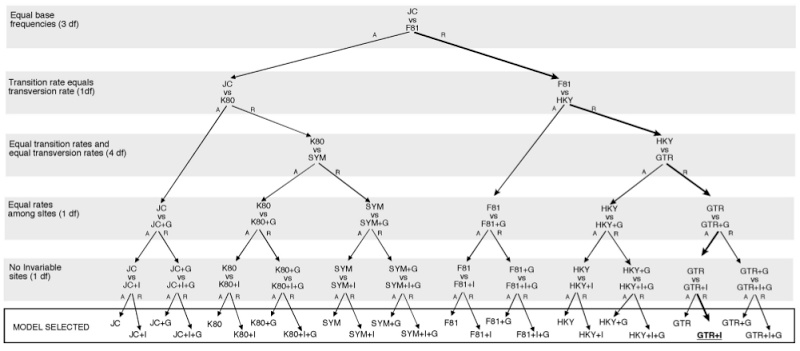
\includegraphics[width=.9\textwidth]{images/hLRT.png}
\end{center}

Figure. Example of a particular forward hierarchy of likelihood ratio tests for 24 models. At any level the null hypothesis (model on top) is either accepted (A) or rejected (R). In this example the model selected is GTR+I.

\subsection{Dynamical Likelihood Ratio Tests (dLRT)}
\label{sec:dlrt}

Alternatively, the order in which parameters are added or removed can be selected automatically. One option to accomplish this is to add the parameter that maximizes a significant gain in likelihood during forward selection, or to add the parameter that minimizes a non-significant loss in likelihood during backward selection \citep{Posada-2001a}. In this case, the order of the tests is not specified a priori, but it will depend on the particular data.

\begin{center}
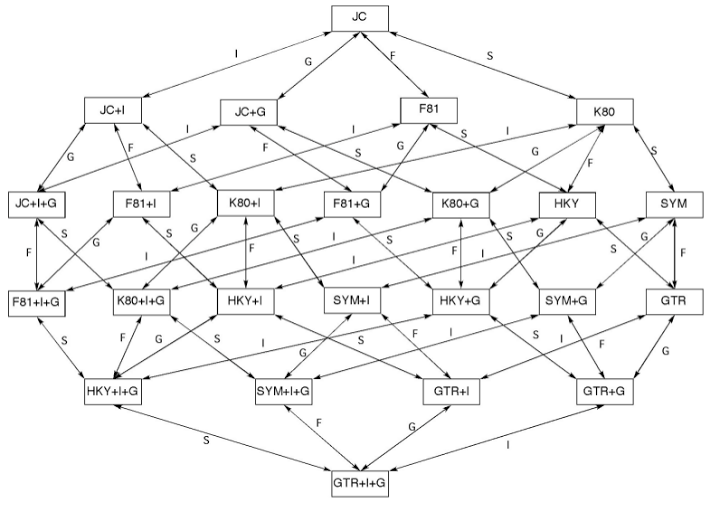
\includegraphics[width=.9\textwidth]{images/dLRT.png}
\end{center}

Figure. Dynamical likelihood ratio tests for 24 models. At any level a hypothesis is either accepted (A) or rejected (R). In this example the model selected is GTR+I. Hypotheses tested are: F = base frequencies; S = substitution type; I = proportion of invariable sites; G = gamma rates.

\subsection{Information Criteria}
\subsubsection{Akaike Information Criterion}
\label{sec:aic}

The Akaike information criterion (AIC, \citep{Akaike-1974} is an asymptotically unbiased estimator of the Kullback-Leibler information quantity \citep{Kullback-1951}. We can think of the AIC as the amount of information lost when we use a specific model to approximate the real process of molecular evolution. Therefore, the model with the smallest AIC is preferred. The AIC is computed as:

\[
AIC=-2l+2k
\]

where l is the maximum log-likelihood value of the data under this model and Ki is the number of free parameters in the model, including branch lengths if they were estimated \emph{de novo}. When sample size ($n$) is small compared to the number of parameters (say, $\frac{n}{K} < 40$) the use of a second order AIC, AICc \citep{Sugiura-1978, Hurvich-1989}, is recommended:

\[
AIC_c=AIC+\frac{(2k(k+1))}{(n-k-1)}
\]

The AIC compares several candidate models simultaneously, it can be used to compare both nested and non-nested models, and model-selection uncertainty can be easily quantified using the AIC differences and Akaike weights (see Model uncertainty below). \citet{Burnham-2003} provide an excellent introduction to the AIC and model selection in general.

\subsubsection{Bayesian Information Criterion}
\label{sec:bic}

An alternative to the use of the AIC is the Bayesian Information Criterion (BIC) \citep{Schwarz-1978}:

\[
BIC=-2l + k log(n)
\]

Given equal priors for all competing models, choosing the model with the smallest BIC is equivalent to selecting the model with the maximum posterior probability. Alternatively, Bayes factors for models of molecular evolution can be calculated using reversible jump MCMC \citep{Huelsenbeck-2004}. We can easily use the BIC instead of the AIC to calculate BIC differences or BIC weights.

\subsubsection{Performance Based Selection}
\label{sec:dt}

\citet{Minin-2003} developed a novel approach that selects models on the basis of their phylogenetic performance, measured as the expected error on branch lengths estimates weighted by their BIC. Under this decision theoretic framework (DT) the best model is the one with that minimizes the risk function:

\[
C_i \approx \sum_{j=1}^n||\hat{B_i} - \hat{B_j}||\frac{e^{\frac{-BIC_j}{2}}}{\sum_{j=1}^R(e^\frac{-BIC_i}{2})}
\]

where 

\[
||\hat{B_i} - \hat{B_j}||^2 = \sum_{l=1}^{2t-3}(\hat{B_{il}} - \hat{B_{jl}})^2
\]

and where t is the number of taxa. Indeed, simulations suggested that models selected with this criterion result in slightly more accurate branch length estimates than those obtained under models selected by the hLRTs \citep{Minin-2003, Abdo-2005}.

\subsection{Model Uncertainty}

The AIC, Bayesian and DT methods can rank the models, allowing us to assess how confident we are in the model selected. For these measures we could present their differences ($\Delta$). For example, for the $i^{th}$ model, the AIC (BIC, DT) difference is:

\[
\Delta_i = AIC_i - min(AIC)
\]

where $min(AIC)$ is the smallest AIC value among all candidate models. The AIC differences are easy to interpret and allow a quick comparison and ranking of candidate models. As a rough rule of thumb, models having $\Delta_i$ within 1-2 of the best model have substantial support and should receive consideration. Models having $\Delta_i$ within 3-7 of the best model have considerably less support, while models with $\Delta_i > 10$ have essentially no support. Very conveniently, we can use these differences to obtain the relative AIC (BIC) weight ($w_i$) of each model:

\[
\omega_i = \frac{e^{\frac{-\Delta_i}{2}}}{\sum_{r=1}^R(e^\frac{-\Delta_r}{2})}
\]

which can be interpreted, from a Bayesian perspective, as the probability that a model is the best approximation to the truth given the data. The weights for every model add to 1, so we can establish an approximate 95\% confidence set of models for the best models by summing the weights from largest to smallest from largest to smallest until the sum is 0.95 \citep{Burnham-1998, Burnham-2003}. This interval can also be set up stochastically (see above ``Model selection and averaging''). Note that this equation will not work for the DT (see the DT explanation on ``Model selection and averaging'').

\subsection{Model Averaging}
\label{sec:model-averaging}

Often there is some uncertainty in selecting the best candidate model. In such cases, or just one when does not want to rely on a single model, inferences can be drawn from all models (or an optimal subset) simultaneously. This is known as model averaging or multimodel inference. See \citet{Posada-2004} and references therein for an explanation of application of these techniques in the context of phylogenetics.

Within the AIC or Bayesian frameworks, it is straightforward to obtain a model-averaged estimate of any parameter \citep{Madigan-1994, Raftery-1996, Hoeting-1999, Wasserman-2000, Burnham-2003, Posada-2003}. For example, a model-averaged estimate of the substitution rate between adenine and cytosine using the Akaike weights for R candidate models would be:

\[
\widehat{\overline{\phi_{A-C}}} = \frac{\sum_{r=1}^R \omega_i I_{\phi_{A-C}}(M_i) \phi_{A-C_i}}{\omega_+(\phi_{A-C})}
\]

where

\[
\omega_+(\phi_{A-C}) = \sum_{i=1}^R \omega_i I_{\phi_{A-C}}(M_i)
\]

and

\[
I_{\phi_{A-C}}(M_i) = \left\{ 
\begin{array}{c l}
1 &  \mbox{$\phi_{A-C}$ is in model $M_i$}\\
0 & \mbox{otherwise}
\end{array}
\right.
\]

Note that need to be careful when interpreting the relative importance of parameters. When the number of candidate models is less than the number of possible combinations of parameters, the presence-absence of some pairs of parameters can be correlated, and so their relative importances.

\subsection{Model Averaged Phylogeny}
\label{sec:consensus}

Indeed, the averaged parameter could be the topology itself, so we could construct a model-averaged estimate of phylogeny. For example, one could estimate a ML tree for all models (or a best subset) and with those one could build a weighted consensus tree using the corresponding Akaike weights. See \citet{Posada-2004} for a practical example.

\subsection{Parameter Importance}
\label{sec:param-importances}

It is possible to estimate the relative importance of any parameter by summing the weights across all models that include the parameters we are interested in. For example, the relative importance of the substitution rate between adenine and cytosine across all candidate models is simply the denominator above, $\omega_+(\phi_{A-C})$
